\chapter{Introduction}

\section{Surgical robotics}

\subsection{Historical Overview of Surgical robotics}

Surgical robotics is a field of Surgery where the surgeon operaties on the patient via a computer, specialised equipment and robotic arms, 
to which the surgical tools needed for the operation are attached. According to surgical bibliography, robotics and laparoscopic procedures are used 
in general surgery, cardiothoracic surgeries, colon surgeries, gynecology, neurosurgery and orthopedics. \\

Robotic mechanisms were first introduced in Medicine, in 1987 with the first laparoscopic surgery of a cholecystectomy. Since then numerous laparoscopic 
operations have been performed and there has been a lot of improvements and innovations in this field. Such surgical operations are characterised as 
\textbf{minimally invasive}, because the surgical incisions made at the patient are very small and thus the probability of infection of the patient during 
or after the operation are very small, the hospitalization time is reduced (which means mean better and more efficient use of hospital resources) and the overall 
recovery of the patient is significantly faster and less painful. \\

However, traditional laparoscopic mechanisms have some downsides as well. First of all, the surgeon should operate in a mirrored-way, meaning that they should 
move at the opposite direction from what they saw at the screen (this effect is also known as the \textbf{fulcrum effect}), in order to reach the desired point of operation. Earlier laparoscopic tools had less 
degrees of freedom, which means less flexibility in motion control. Moreover these systems provided limited touch sensibility and feedback to the doctor they 
were very susceptible to the surgeon's micro movements and tremble. \\

The first application of robotics in Surgery appears in 1985, when Kwoh et al. \cite{Shao1985ANC} used a \textbf{PUMA 560}, a standard industrial robotic arm, to perform a neurosurgical biopsy, 
where the biopsy needle was inserted in the brain and guided with the help of Computed Tomography. This successful application was followed by the \textbf{PROBOT} surgical robot \cite{Probot1992}, 
which was developed at the Imperial College and used in a prostatectomy operation. Another example of an early surgery robot was the \textbf{ROBODOC} system \cite{Robodoc} developed by Integrated Surgical Supplies 
in Sacramento California, which was the first to be used in orthopedics for a hip replacement surgery and was also the first to be approved by the FDA (Food \& Drug Administration, organization responsible 
for medical devices, drugs etc.).

\begin{center}
\begin{figure}[!htb]
\centering
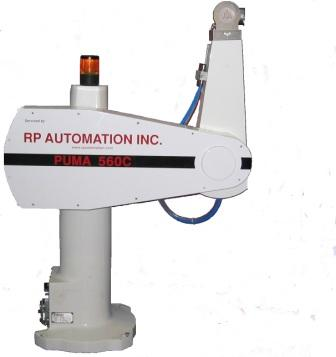
\includegraphics{images/Puma560.jpg}\\
\caption{The PUMA 560 robotic arm, which was the first to be used in surgery robotics in 1985}
\end{figure}
\end{center}

Some other important surgery robots are listed below:
\begin{itemize}
\item \textbf{AESOP\textsuperscript \textregistered Endoscope Positioner}: A voice controlled endoscopic system
\item \textbf{HERMES\textsuperscript \textregistered Control Center}
\item \textbf{daVinci Surgical System\textsuperscript \textregistered}: One of the most popular surgery robots and most used 
in hospitals. It is a master-slave system, which means that the operation commands are sent uni-directionally from the master 
console, which is controlled by the surgeon, and are executed by the robot. It also comes with a high definition 3D video feed 
and advanced manipulator system, one for each hand, called EndoWrist\textsuperscript \textregistered. It is officially approved 
by the FDA for laparoscopic surgeries.
\item \textbf{SOCRATES Robotic Telecollaboration System}
\item \textbf{Raven-II} \cite{Raven2}: An open platform for collaborative research on surgical robotics.
\item \textbf{Monarch\textsuperscript \texttrademark Platform} by Auris Health Inc., an endoscopic system for robotic-assisted 
bronchoscopy
\end{itemize}

\begin{center}
\begin{figure}[!htb]
\centering
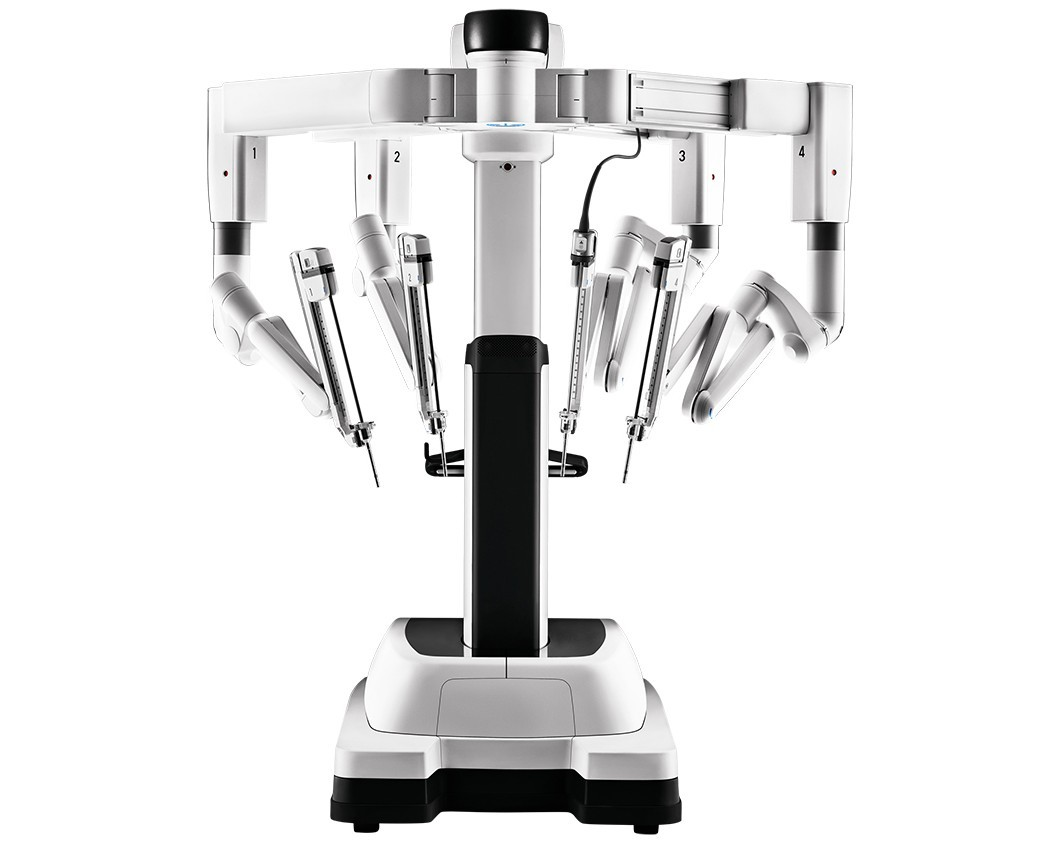
\includegraphics[width=0.7\textwidth]{images/intuitive-da-vinci-xi-patient-cart-front-view-1060867-lo-res.jpg}\\
\caption{DaVinci Xi, \textsuperscript \textcopyright 2020 Intuitive Surgical, Inc. Patient Cart with the robotic arms that control the surgical tools}
\end{figure}
\end{center}

\begin{center}
\begin{figure}[!htb]
\centering
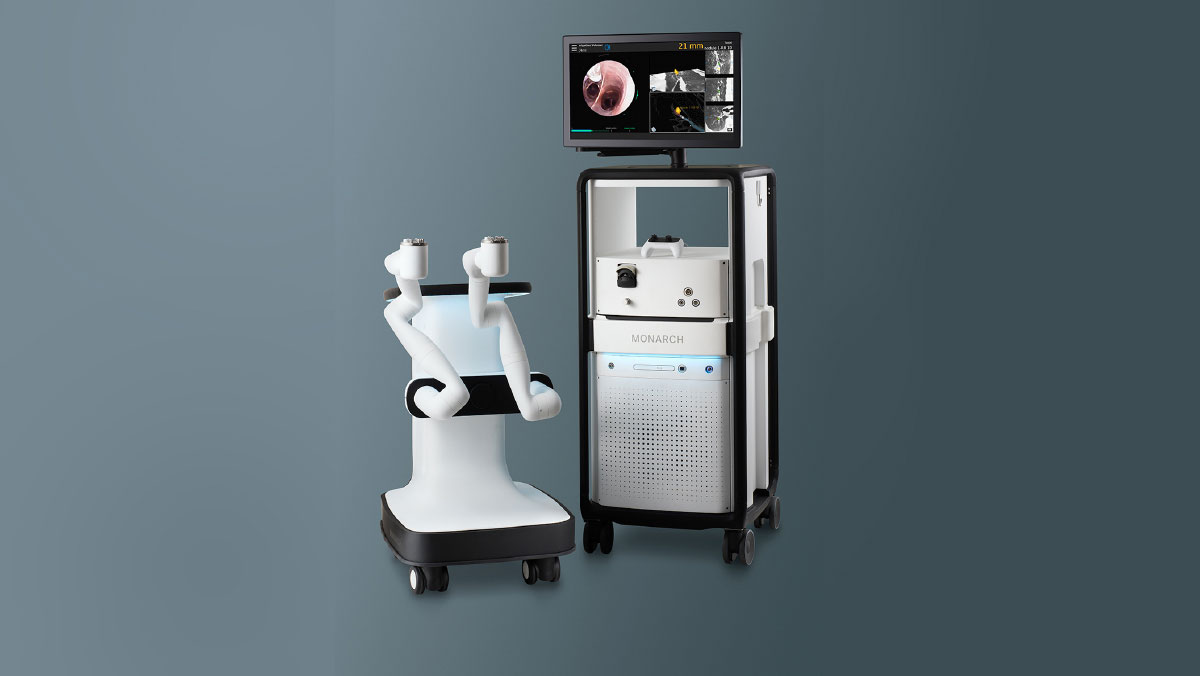
\includegraphics[width=0.8\textwidth]{images/Moarch_Platform_1200_x_676_1_.jpg}\\
\caption[The Monarch\textsuperscript \texttrademark Platform endoscopic system]{The Monarch\textsuperscript \texttrademark Platform endoscopic system \footnotemark}
\end{figure}
\end{center}
% How to use caption with footnote https://tex.stackexchange.com/questions/10181/using-footnote-in-a-figures-caption 
\footnotetext{\url{https://www.aurishealth.com/patients/robotic-bronchoscopy-patient-about-monarch-platform }}


\subsection{Surgical Robotics Procedure}

The robotic surgery procedure starts with total anesthesia of the patient. Then the surgeon makes small incisions at the anatomical region of interest, where the procedure will take place. Through 
these small incisions special tubes, called trocars, are mounted, through which the laparoscopic tools are inserted. After the patient is prepared and after the patient cart, which carries the robotic arms, 
is successfully positioned and callibrated, the surgeon sits on a console, from where they control they robot via special sensitive joysticks. The surgeon has vision access (often in 3D) to the surgical site via a
small endoscopic camera and the video is displayed on the console. In some cases, the surgeon gets force feedback from the joysticks via haptic mechanisms. Haptic force feedback is very important for the doctor 
in order to have a better sense of the anatomy and the surgical site, and it has gained a lot of interest in the reasearch community.

\begin{center}
\begin{figure}[!htb]
\centering
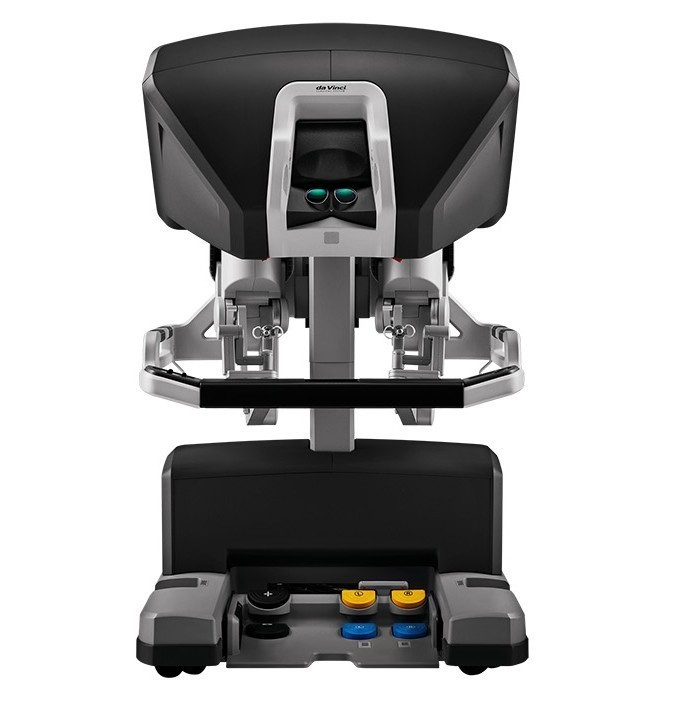
\includegraphics[width=0.5\textwidth]{images/intuitive-davinci-console-front-lowres.jpg}\\
\caption[DaVinci Xi \textsuperscript \textcopyright 2020 Intuitive Surgical, Inc. Surgeon Console]{DaVinci Xi \textsuperscript \textcopyright 2020 Intuitive Surgical, Inc. Surgeon Console \footnotemark}
\end{figure}
\end{center}
\footnotetext{\url{https://www.intuitive.com/en-us/about-us/press/press-resources}}


\subsection{Advantages \& Disadvantages of Surgical robotics}

Surgical robotics have a huge impact in Medicine and Healthcare in general. Some of the advantages are the following:
\begin{itemize}
\item \textbf{Minimally Invasive Procedures} which means
	\begin{itemize}
	\item Smaller incisions
	\item Less blood loss
	\item Reduced risk of inpatient infection
	\item Less pain
	\item Faster patient recovery
	\end{itemize}
\item Increased \textbf{precision} and reduced human errors
	\begin{itemize}
	\item Smooth and precise movements
	\item Detection and correction of errors caused by hand tremble
	\end{itemize}
\item \textbf{No fulcrum effect} and intuitive manipulation of surgical tools
\item \textbf{Haptic feedback}. This technology uses small mechanical forces and vibrations to give the user the sense of touch or force. Force feedback gives the ability to the surgeon to understand the 
mechanical properties of the tissue they operate on, such as resistance and elasticity, and thus distinguish between healthy from unhealthy tissue
\item \textbf{Teleoperation} (currently in the same room only): the surgeon operates while they sit on a special \textbf{ergonomic} console, which makes 
the long procedures more comfortable and efficient.
\end{itemize} 

\section{Problem statement}

The goal of this thesis is to design the kinematic models and algorithms necessary for a robotic arm to detect, pick and manipulate a laparoscopic surgical tool. To achieve these goals the robotic arm must 
successfully do the following:
\begin{itemize}
\item Use computer vision to detect the scene and laparoscopic tools and with the help of stereoscopic vision, calculate the position and orientation of the center of mass of each tool, with respect to the 
universal reference frame
\item Calculate the contact points on the tool, on which the fingers of the gripper will be placed, so that there is a firm grasp (force closure)
\item Calculate the path from the tools' table to the surgical site table
\item Calculate the trajectory that needs to be executed when the tool is inserted in the trocar. This is a special type of trajectory, because the motion is constrained and is known in the bibliography as
a \textbf{Remote Center of Motion} (RCM) control. The constraint is that, at each time one point of the inserted tool must coincide with the RCM point (this point will also be referenced in this thesis as the center of the 
trocar, or the fulcrum reference frame point).
\end{itemize}

\section{Bibliography Overview}

\section{Methodology \& Approach}

Robotics and especially surgery robotics is a multi-disciplinary field and a robot has many subsystems. A very important approach to successfully design a robotic arm to execute a surgery task is to subdivide the 
task in multiple smaller submodules and design, implement and test each submodule separately and then combine them together for end-to-end testing.

\begin{center}
\begin{figure}[!htb]
\centering
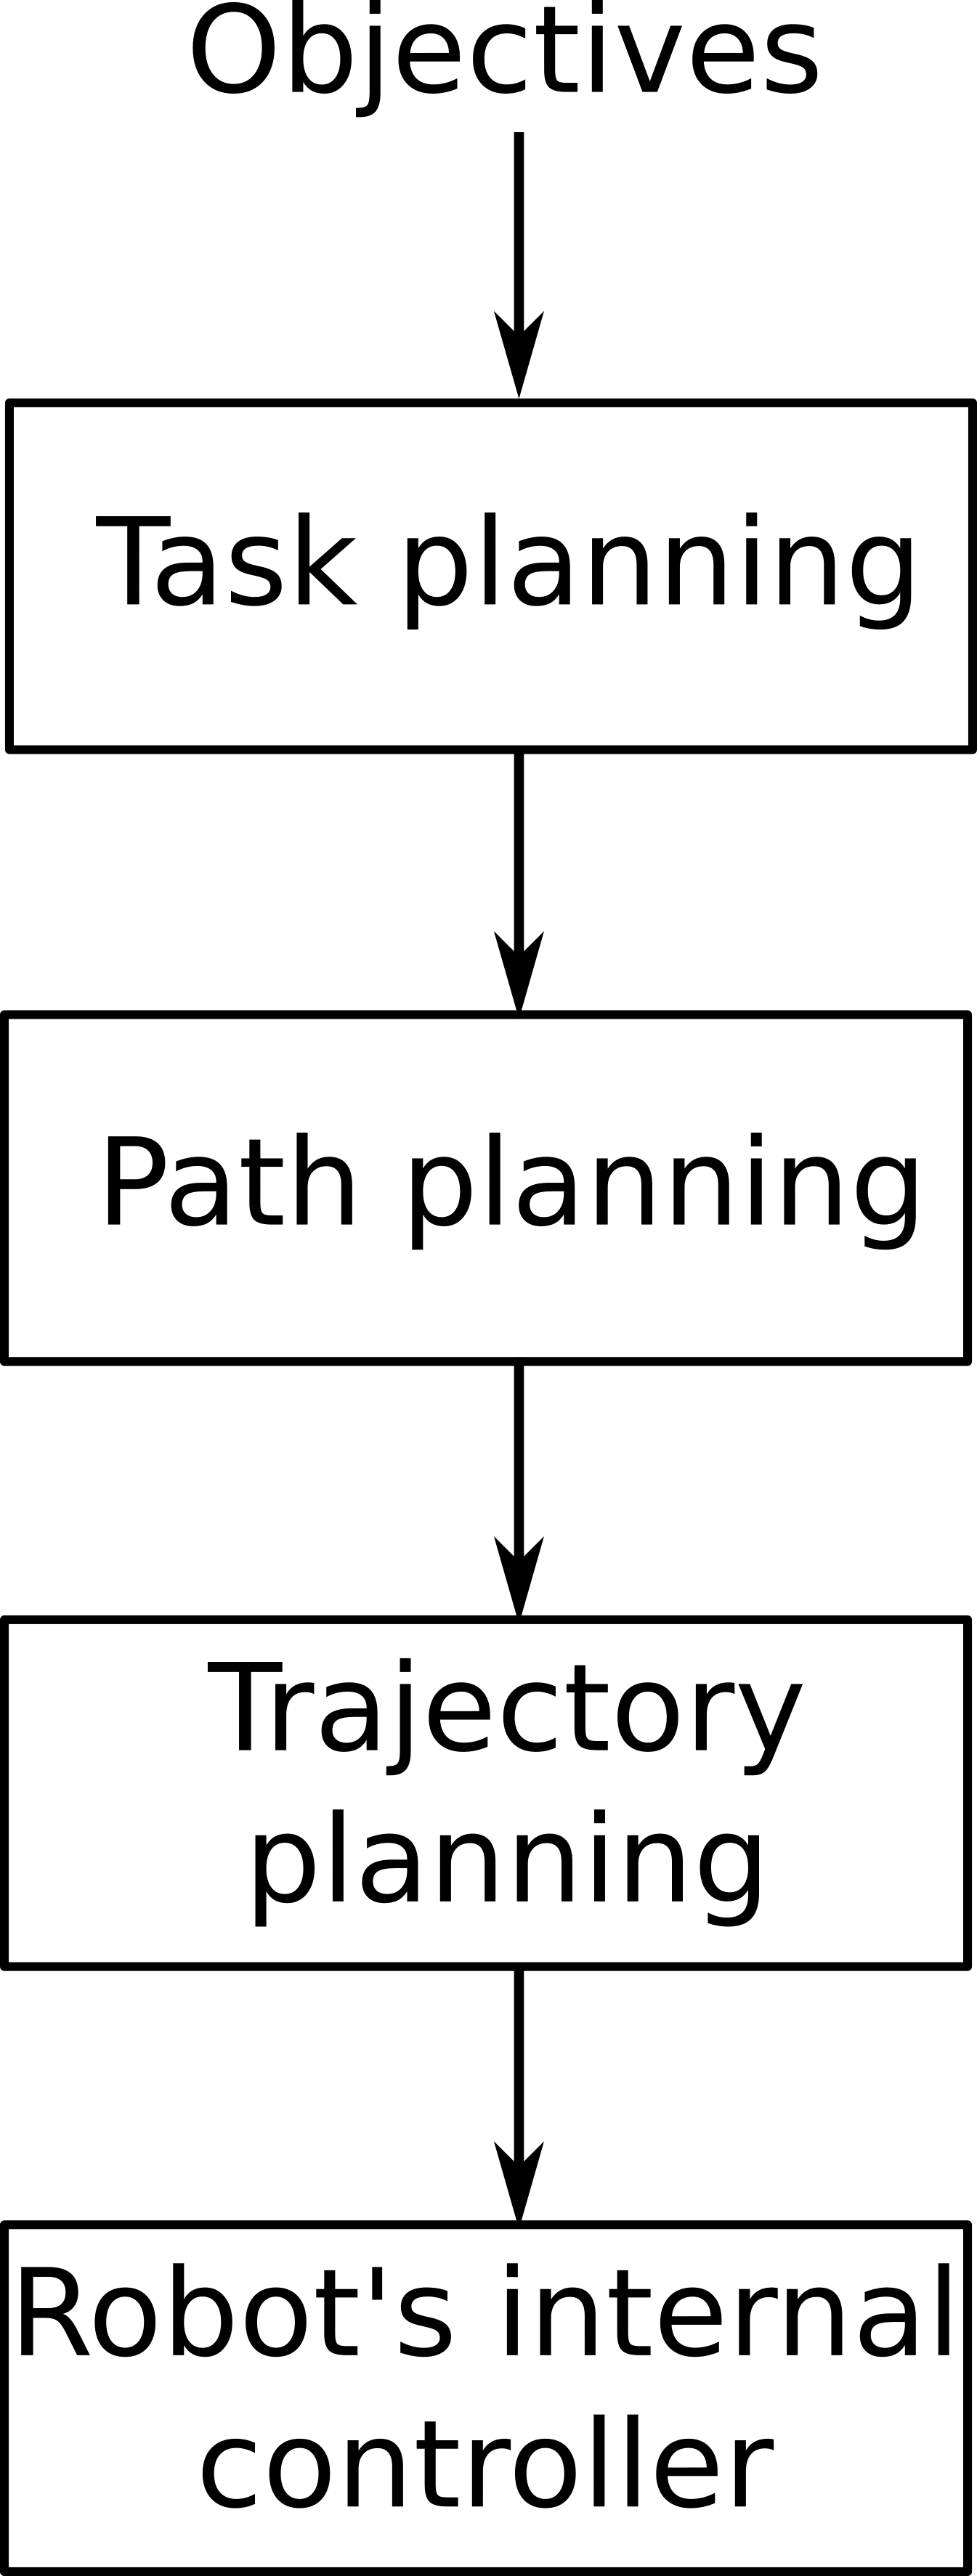
\includegraphics[width=0.15\textwidth]{images/motion-planning.png}\\
\caption{Motion planning pipeline}
\end{figure}
\end{center}

\textbf{Tools \& Software used in this thesis}:
\begin{itemize}
\item Matlab \& Matlab toolboxes: ROS Toolbox, Robotics Toolbox
\item ROS Framework
\item MoveIt
\item Gazebo simulator
\item VREP simulator
\item OpenCV
\end{itemize}

\textbf{Methodology of conducting this thesis}:
\begin{itemize}
\item Mathematical calculations for Kinematics and Motion planning
\item Mathematics validation with Matlab
\item Quick prototyping and testing with Matlab and/or VREP
\item Implementation in ROS frameworks, by splitting the end-to-end robotic operation in smaller 
experiments and tasks
\end{itemize}

\begin{center}
\begin{figure}[!htb]
\centering
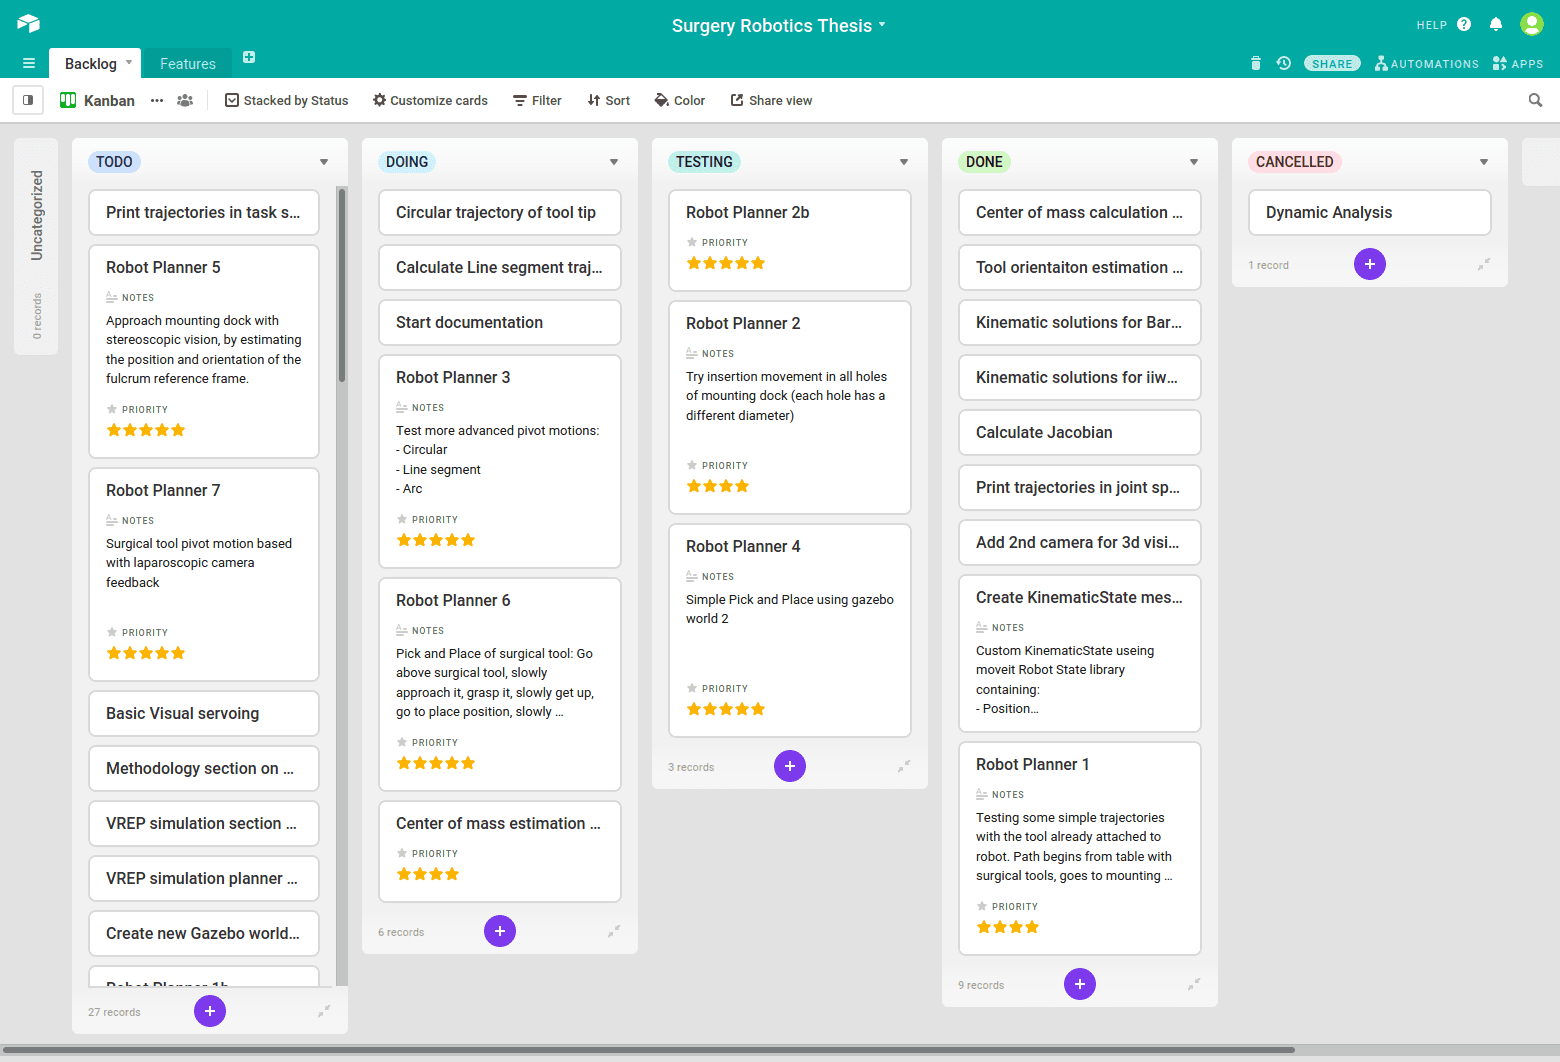
\includegraphics[width=0.7\textwidth]{images/task-backlog-airtable.png}\\
\caption{Kanban view of backlog tasks to organize all features, requirerements and tasks needed to complete this thesis. The tool used to keep track of all tasks is Airtable}
\end{figure}
\end{center}

To quickly test out ideas on how to build the robot's environment and the simulation layout, as well as some simple trajectories, the CoppeliaSim simulator software was used (also known previously as VREP).
CoppeliaSim allowed to do quick prototyping using the intuitive drag-and-drop interface and the embedded scripts, before implementing the actual simulation in ROS which is more complex and time-consuming (but also more
feature-rich).

\begin{center}
\begin{figure}[!htb]
\centering
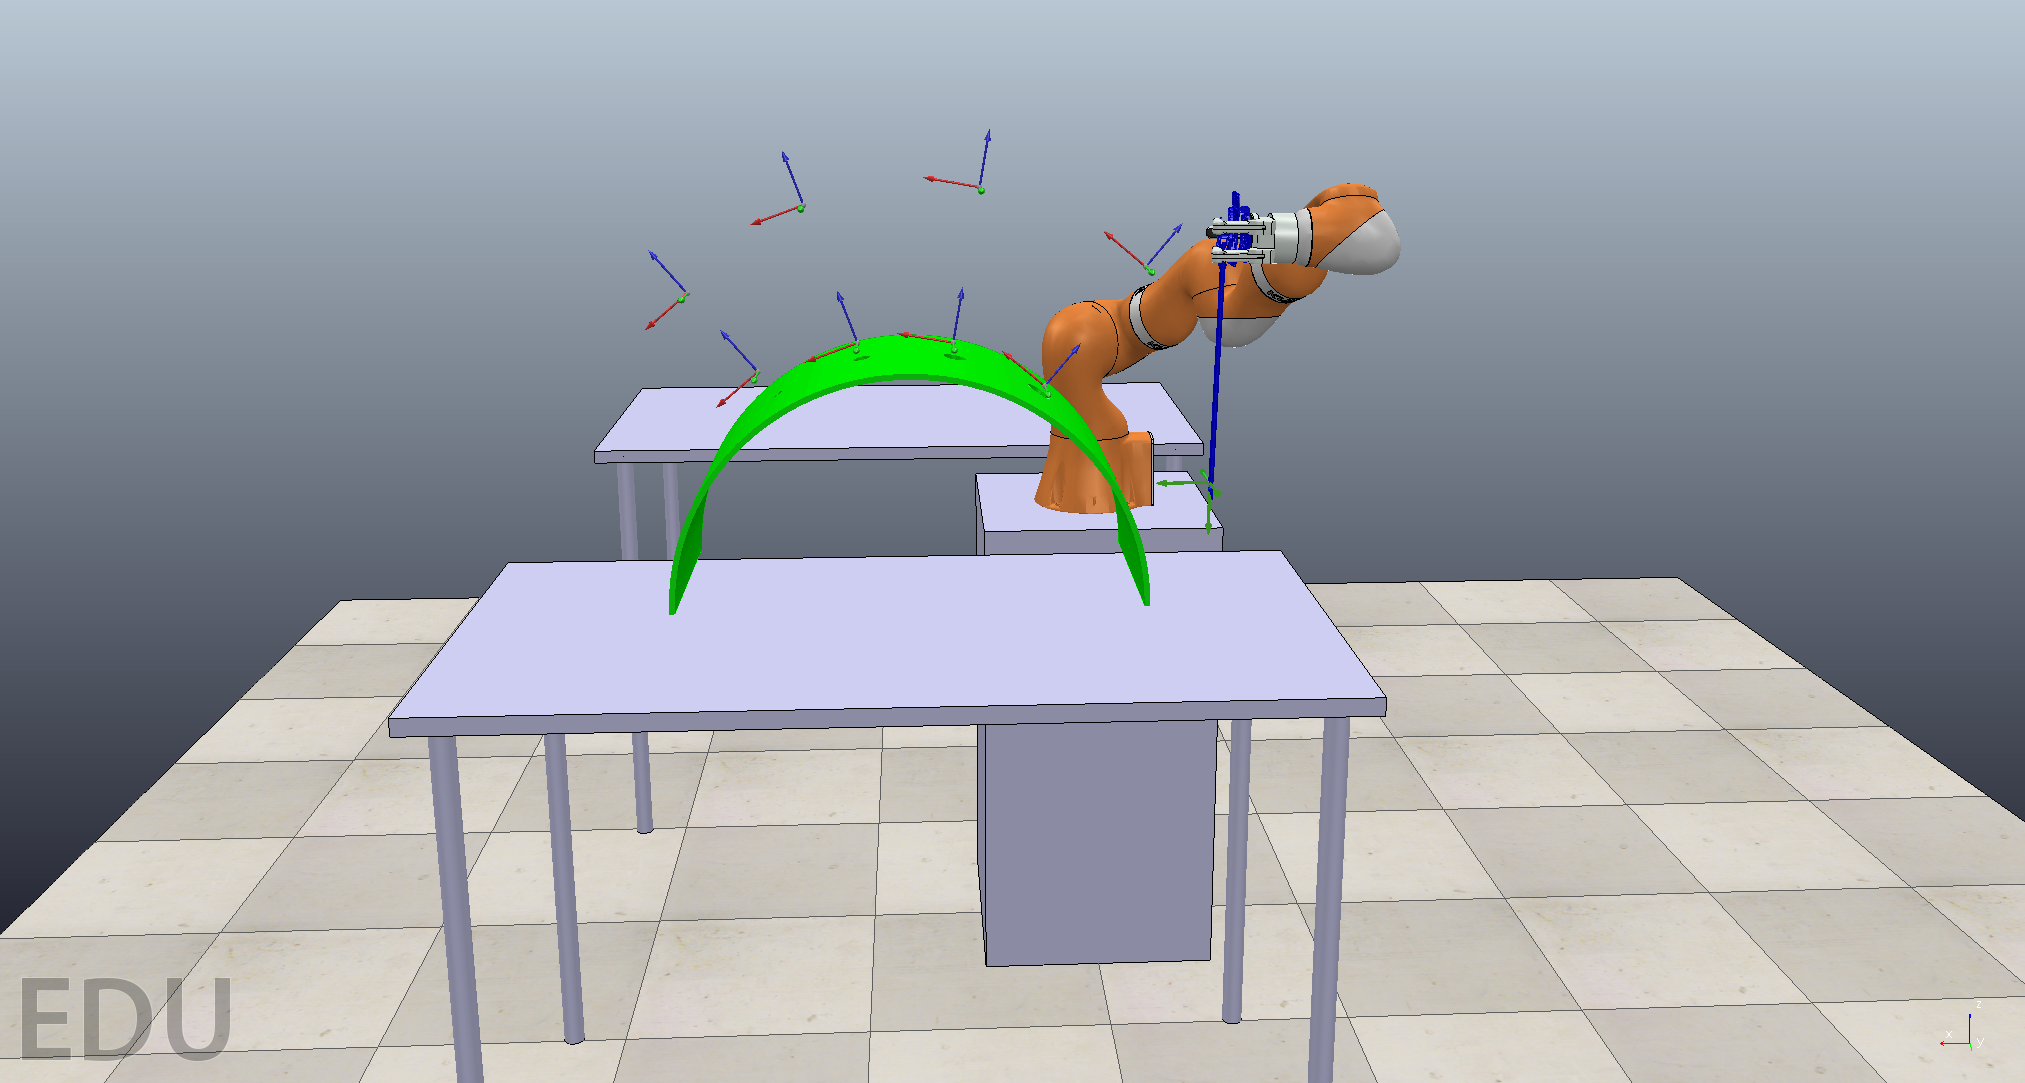
\includegraphics[width=\textwidth]{images/quick-vrep-prototyping.png}\\
\caption{Quick Prototyping using the VREP (CoppeliaSim) simulation environment}
\end{figure}
\end{center}